\documentclass[upright, contnum]{umemoria}
\depto{Departamento de Ingeniería Eléctrica}
\author{Rodrigo Javier Pérez Dattari}
\title{Interactive Learning with Corrective Feedback for Continuous-Action Policies based on Deep Neural Networks}
\auspicio{Proyecto FONDECYT 1161500}
\date{2019}
\guia{Javier Ruiz del Solar}
\carrera{Magíster en Ciencias de la Ingeniería, Mención Eléctrica}
\carreraeng{Master of Engineering Sciences in Electrical Engineering}
\memoria{Tesis para optar al Grado de \break  Magíster en Ciencias de la Ingeniería, Mención Eléctrica\break \break
Memoria para optar al Título de Ingeniero Civil Eléctrico}
\comision{Javier Ruiz del Solar, Felipe Tobar, Nicolás Navarro-Guerrero}

\usepackage{lipsum}

\usepackage[utf8]{inputenc}
\usepackage[T1]{fontenc}
\usepackage{color}
\usepackage{titlesec}
\usepackage[noend]{algpseudocode}
\usepackage{amsmath}
\usepackage{algorithm}
\usepackage{subfig}
\usepackage{blindtext, graphicx}
\usepackage{color}
\definecolor{mygray}{RGB}{200, 200, 200}
\definecolor{mygreen}{RGB}{1, 200, 1}
\definecolor{lightgray}{gray}{0.8}
\definecolor{lightlightgray}{gray}{0.9}
\newcommand{\new}[1]{\color{blue}{#1}\color{black}}
\newcommand{\replace}[1]{\color{mygray}{#1}\color{black}} % replace text, or not needed
\newcommand{\remove}[1]{\color{red}{#1}\color{black}}
\newcommand{\comment}[1]{\color{mygreen}{#1}\color{black}}
\newcommand{\note}[1]{\color{red}\textbf{{#1}}\color{black}}

\titlespacing*{\section}{0pt}{\baselineskip}{\baselineskip}
\titlespacing*{\subsection}{0pt}{\baselineskip}{\baselineskip}
\titlespacing*{\subsubsection}{0pt}{\baselineskip}{\baselineskip}
\DeclareMathOperator*{\argmax}{arg\,max}
\DeclareMathOperator*{\argmin}{arg\,min}

\begin{document}

\frontmatter
\maketitle

\begin{abstract}
El Aprendizaje Reforzado Profundo (DRL) se ha transformado en una metodología poderosa para resolver problemas complejos de toma de decisión secuencial. Sin embargo, el DRL tiene varias limitaciones cuando es usado en problemas del mundo real (p.ej. aplicaciones de robótica). Por ejemplo, largos tiempos de entrenamiento (que no se pueden acelerar) son requeridos, en contraste con ambientes simulados, y las funciones de recompensa pueden ser difíciles de especificar/modelar y/o computar. Más aún, el traspaso de políticas aprendidas en simulaciones al mundo real no es directo ("reality gap"). Por otro lado, métodos de aprendizaje de máquinas basados en la transferencia de conocimiento humano a un agente han mostrado ser capaces de obtener políticas con buenos desempeños sin necesariamente requerir el uso de una función de recompensa, siendo eficientes en lo que respecta al tiempo.

En este contexto, en esta tesis se introduce una estrategia de Aprendizaje Interactivo de Máquinas (IML) para entrenar políticas modeladas como Redes Neuronales Profundas (DNNs), basada en retroalimentación correctiva humana con un método llamado D-COACH. Se combina Aprendizaje Profundo (DL) con el método Asesoramiento Correctivo Comunicado por Humanos (COACH), en donde humanos no expertos pueden entrenar políticas corrigiendo las acciones que va tomando el agente en ejecución. El método D-COACH tiene el potencial de resolver problemas complejos sin necesitar de muchos datos o tiempo. Resultados experimentales validan la eficiencia del método propuesto en plataformas simuladas y del mundo real, en espacios de estados de baja y alta dimensionalidad, mostrando la capacidad de aprender políticas en espacios de acción continuos de manera efectiva.

El método propuesto mostró resultados particularmente interesantes cuando políticas parametrizadas con Redes Neuronales Convolucionales (CNNs) fueron usadas para resolver problemas con espacios de estado de alta dimensionalidad, como pixeles desde una imagen. Al usar CNNs, los agentes tienen la capacidad de construir valiosas representaciones del estado del ambiente sin la necesidad de hacer ingeniería de características por el lado del diseñador (lo que era siempre necesario en el Aprendizaje Reforzado (RL) clásico). Estas propiedades pueden ser muy útiles en robótica, ya que es común encontrar aplicaciones en donde la información adquirida por los sensores del sistema es de alta dimensionalidad, como imágenes RGB. Darles la habilidad a los robots de aprender desde datos del alta dimensionalidad va a permitir aumentar la complejidad de los problemas que estos pueden resolver.

A lo largo de esta tesis se proponen y validan tres variaciones de D-COACH. La primera introduce una estructura general para resolver problemas de estado de baja y alta dimensionalidad. La segunda propone una variación del primer método propuesto para problemas de estado de alta dimensionalidad, reduciendo el tiempo y esfuerzo de un humano al entrenar una política. Y por último, la tercera introduce el uso de Redes Neuronales Recurrentes para añadirle memoria a los agentes en problemas con observabilidad parcial.

\end{abstract}

\begin{abstract_eng}
Deep Reinforcement Learning (DRL) has become a powerful methodology to solve complex decision making problems. However, DRL has several limitations when used in real-world problems (e.g., robotics applications). For instance, long training times (that cannot be accelerated) are required in contrast to simulated environments, and reward functions may be hard to specify/model and/or to compute. Moreover, the transfer of policies learned in a simulator to the real-world has limitations (reality gap). On the other hand, machine learning methods that rely on the transfer of human knowledge to an agent have shown to be time efficient for obtaining well performing policies and do not require a reward function.

In this context, this thesis proposes an alternative Interactive Machine Learning (IML) strategy for training Deep Neural Network (DNN) policies based on human corrective feedback, with a method called Deep COACH (D-COACH). Deep Learning is combined with the COrrective Advice Communicated by Humans (COACH) framework, in which non-expert humans shape policies by correcting the agent’s actions during execution. The D-COACH framework has the potential to solve complex problems without much data or time required. Experimental results validated the efficiency of the proposed framework in simulated and real-world platforms, with state spaces of low and high dimensionality, showing the capacity to successfully learn policies for continuous action spaces. 

The proposed framework showed particularly interesting results when learning policies parameterized with Convolutional Neural Networks (CNNs) for high-dimensional state spaces, such as raw pixels from an image. By using CNNs, agents are given the possibility to build rich state representations of the environment without feature engineering on the side of the designer (which was always necessary in classical RL). These properties can be very useful in robotics, since it is common to find applications with high-dimensional observations, such as RGB images. Giving robots the ability to learn from such high-dimensional data will allow to scale up the complexity of what robots are able to do.

In this thesis three variations of D-COACH are proposed and validated. The first one introduces a general structure for solving problems with low-dimensional and high-dimensional state spaces. The second one proposes a variation of the first approach for high-dimensional state problems, reducing the time and effort of a human for training a policy. And finally, the third variation introduces the use of Recurrent Neural Networks for adding memory to agents in problems with partial observability.
\end{abstract_eng}


\begin{dedicatoria}
A mi abuelo Ernesto
\end{dedicatoria}

\begin{thanks}

\end{thanks}

\cleardoublepage
\tableofcontents
\cleardoublepage
\listoftables
\cleardoublepage
\listoffigures

\mainmatter

\begin{intro}
\section{Motivation and Problem Statement}
In  recent years outstanding results in complex decision-making problems have been obtained with Deep Reinforcement Learning (DRL). State of the art algorithms have solved problems with large state spaces and discrete action spaces, such as playing Atari games \cite{atari}, or beating the world champion in GO \cite{Silver2016}, along with low level simulated continuous control tasks in environments such as the ones included in the OpenAI Gym \cite{brockman2016openai} and the DeepMind Control Suite \cite{tassa2018deepmind}. Learning policies, parameterized with Convolutional Neural Networks (CNN) for high-dimensional state spaces, such as raw images, gives agents the possibility to build rich state representations of the environment without feature engineering on the side of the designer (which was always necessary in classical RL). These properties can be really useful in complex robotics problems, giving robots the ability to solve problems using raw visual information. 

Nevertheless, DRL has several limitations when used to address real world systems \cite{Gu2017}. For instance, DRL algorithms require large amounts of data, which means long training times that in contrast to simulated environments cannot be accelerated with more computational power. If somehow this shortcoming was addressed, sometimes the reward function would still pose a problem as it is hard to specify/model and/or to compute in many cases in the real-world. For instance, sometimes additional perception capabilities to the ones of the agent are needed for computing the reward function, since in theory the reward is given ``by the environment``, not be the agent.

In this regard, the transfer of knowledge learned in a simulator to the real-world is a typical solution. However the mismatch between the virtual and real environment, known as ``Reality Gap``, is often problematic \cite{koos2013transferability}. This results in agents that do not perform at their best in the real-world. Thus, it would be preferable to learn/fine-tune policies directly in the real-world.

On the other hand, machine learning methods that rely on the transfer of human knowledge to an agent have shown to be time efficient for obtaining good performance policies. Moreover, some methods do not need expert human teachers for training high performance agents \cite{akrour2011preference,Knox:2009:ISA:1597735.1597738,Celemin2018AnInteractive}. This is why they appear to be good candidates to tackle the DRL real-world issues mentioned before. 

Therefore, in this work, we study the use of human corrective feedback during task execution, to learn policies with high dimensional state spaces, in continuous action problems using CNNs. Our work extends D-COACH \cite{perez2018interactive}, which is a Deep Learning (DL) based extension of the COrrective Advice Communicated by Humans (COACH) framework \cite{Celemin2018AnInteractive}. In the original D-COACH formulation, a demonstration session is required, at the beginning of the training process, for tuning the convolutional layers used for state dimensionality reduction. After that, a fully connected network policy (connected to the previously trained encoder) is interactively trained during task execution with the human corrective feedback, similarly to the human-agent interaction of the original COACH.

In this paper we introduce an enhanced version of D-COACH, which eliminates the need of demonstration sessions and trains the whole CNN simultaneously, reducing the time and effort of the user/coach for teaching a policy.  In D-COACH no reward functions are needed, and the amount of learning episodes are significantly reduced in comparison to alternative DRL approaches. Enhanced D-COACH is validated in three different problems through simulations and real-world scenarios. In each problem, %two % 
the original and enhanced D-COACH are analyzed and compared with the DDPG method. 

ISER

Deep Reinforcement Learning (DRL) has obtained unprecedented results in decision-making problems, such as playing Atari games \cite{Mnih2013}, or beating the world champion in GO \cite{Silver2016}. Nevertheless, in robotic problems, DRL is still limited in applications with real-world systems \cite{Gu2017}. Most of the tasks that have been successfully addressed with DRL have two common characteristics: 1) they have well-specified reward functions, and 2) they require large amounts of trials, which means long training periods (or powerful computers) to obtain a satisfying behavior. These two characteristics can be problematic in cases where 1) the goals of the tasks are poorly defined or hard to specify/model (reward function does not exist), 2) the execution of many trials is not feasible (real systems case) and/or not much computational power or time is available, and 3) sometimes additional external perception is necessary for computing the reward/cost function. 

On the other hand, Machine Learning methods that rely on transfer of human knowledge, Interactive Machine Learning (IML) methods, have shown to be time efficient for obtaining good performance policies and may not require a well-specified reward function; moreover, some methods do not need expert human teachers for training high performance agents \cite{akrour2011preference,Knox:2009:ISA:1597735.1597738,Celemin2018AnInteractive}. In previous years, IML techniques were limited to work with low-dimensional state spaces problems and to the use of function approximation such as linear models of basis functions (choosing a right basis function set was crucial for successful learning), in the same way as RL. But, as DRL have showed, by approximating policies with Deep Neural Networks (DNNs) it is possible to solve problems with high-dimensional state spaces, without the need of feature engineering for preprocessing the states. If the same approach is used in IML, the DRL shortcomings mentioned before can be addressed with the support of human users who participate in the learning process of the agent.

This work proposes to extend the use of human corrective feedback during task execution to learn policies with state spaces of low and high dimensionality in continuous action problems (which is the case for most of the problems in robotics) using deep neural networks.

We combine Deep Learning (DL) with the corrective advice based learning framework called COrrective Advice Communicated by Humans (COACH) \cite{Celemin2018AnInteractive}, thus creating the Deep COACH (D-COACH) framework. In this approach, no reward functions are needed and the amount of learning episodes is significantly reduced in comparison to alternative approaches. D-COACH is validated in three different tasks, two in simulations and one in the real-world.
\section{Objectives}
\subsection{General Objectives}
\subsection{Specific Objectives}
\section{Hypotheses}
\section{Contribution}
\section{Outline}
\end{intro}
\chapter{Theoretical Framework}
\section{Machine Learning}

Machine Learning (ML) is a discipline that studies ways of finding patterns in data by learning from experience. What this mean, is that an algorithm in charge of accomplishing an specific task is able to progressively improve its performance (learn) by comparing its output with data (experience) in a way that indicates how good/bad is doing. If the algorithm is doing good, then the learning process is finished. If is not doing so good, then the algorithm updates its parameters to match (if possible) its output with what is expected.   
\subsection{Deep Learning}

\subsubsection{Autoencoder}

\section{Policy Learning}
\note{POLICY DESCRIPTION}
\subsection{Reinforcement Learning}
\subsubsection{Deep Reinforcement Learning}
\subsection{Learning from Demonstration}
\subsubsection{The Correspondence Problem}
\subsection{Interactive Learning}
\subsubsection{Evaluative Feedback}
\subsubsection{Corrective Feedback}
\section{Function Approximation}
\subsection{Linear Model of Basis Functions}
\subsection{Artificial Neural Networks}
\section{COrrective Advice Communicated by Humans (COACH)}
\chapter{Using Neural Networks to Enhance COACH}
\section{Deep COACH}

\chapter{Enhancing D-COACH for High-Dimensional State Problems}
\section{Overview}

In this chapter we introduce  D-COACH ON, a variation of D-COACH OFF for problems with high-dimensional state spaces. This is motivated by the limitation that D-COACH OFF presents when learning state representations. Recording a database with observations of the environment and training an autoencoder in an offline step can be time consuming and not robust to changes in the environment. Thus, it would be desirable to have a version of D-COACH that eliminates this offline step, learning everything in a single interaction step, as the original COACH does. Hence, an algorithm capable of training all the parameters of the network interactively from scratch. 

\section{Online State Representation Learning}
In order to obtain an algorithm capable of learning interactively from scratch we need to make the networks to converge faster. In the former chapter, an autoencoder was used to learn a low-dimensional representation of high-dimensional states in an offline learning process. In this chapter, we propose to use the autoencoder learning criteria during the interactive learning process, such that both networks (the policy and the autoencoder) share the convolutional layers of the encoder, as shown in Fig.~\ref{fig:msim}.

\begin{figure}[H]
    \centering
    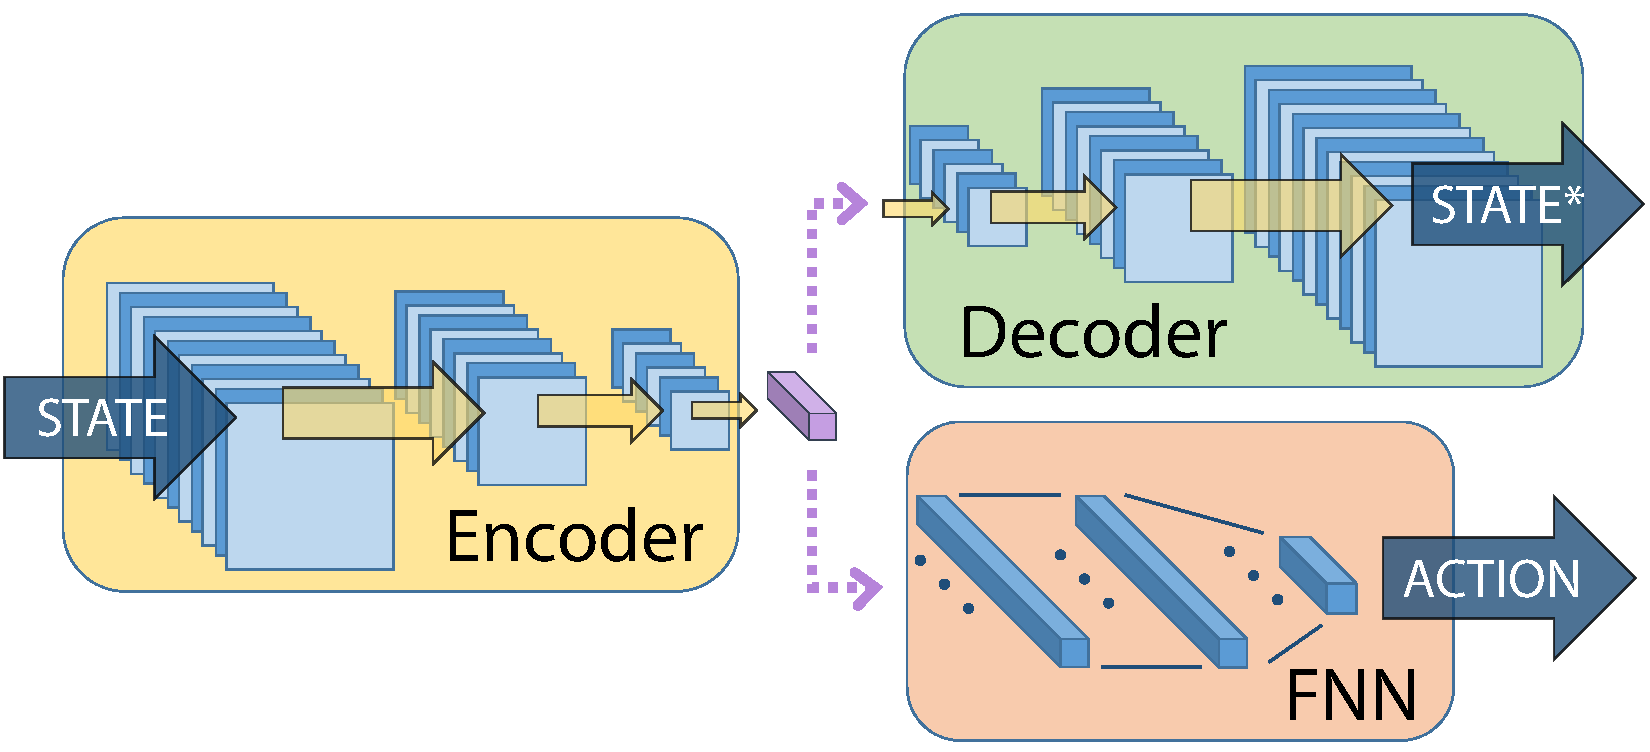
\includegraphics[width=0.6\linewidth]{imagenes/cap2/m2.pdf}
    \caption{D-COACH ON: Online state representation learning. The state representation is shared between the autoencoder and the policy training.}
    \label{fig:msim}
\end{figure}

The policy network has the convolutional layers at the input, followed by a second part that is a fully-connected layer, then this network maps STATE into ACTION, while the autoencoder network involves the computation from STATE to STATE$^{*}$, wherein  STATE$^{*}$ is the reconstructed image at the output of the decoder. Autoencoding is seen as an additional auxiliary criteria for training the state representation of the policy online. 

%So, in addition to the loss function for predicting the policy based on the data generated by the human corrections, it also includes the loss function of the reconstruction at the output of the autoencoder, based on the same data stored during the human corrections. 

\section{The Algorithm}
Algorithm \ref{algorithm:EnDeepCOACH} describes D-COACH ON. The algorithm first sets the hyper-parameters like the magnitude of the error (Equation \ref{eq:error}), and the ones used for the corrections replay. In cases when the teacher advises a correction (line 6, Algorithm \ref{algorithm:EnDeepCOACH}), the subsequent lines are evaluated, wherein the policy network is updated along with the autoencoder network.

Two different updates are computed, one for the layers involved in the policy computation, and another for the layers of the autoencoder. When feedback is given by the teacher, the \textbf{update} \emph{policy} instruction updates the policy network for the current time step only using this last received feedback. Subsequently, the \emph{batch\_update} subroutine is called. This subroutine is in charge of updating the policy and the autoencoder by sampling a mini-batch from the replay buffer. The \emph{batch\_update} subroutine is also called every $b$ time steps (line 15, Algorithm \ref{algorithm:EnDeepCOACH}).

The \emph{batch\_update} subroutine is described in Algorithm \ref{algorithm:batch_update}. When this subroutine is called, the autoencoder is updated only if its reconstruction error in the last \emph{m} observations (MSE between STATE and STATE$^{*}$) is greater than a threshold $\epsilon$ (line 4, Algorithm \ref{algorithm:batch_update}). Otherwise, the autoencoder is not updated and the convolutional layers of the encoder are frozen. As a consequence, the instruction \textbf{update} \emph{policy} in lines 3 (Algorithm \ref{algorithm:batch_update}) and 10 (Algorithm \ref{algorithm:EnDeepCOACH}) only modifies the non-convolutional layers of the policy. 

The condition for training the autoncoder is used for avoiding conflicts in the gradients of both cost functions, so when the latent vector of the autoencoder is considered a good smaller representation of the state, the gradient of the policy must be prevented from harming the learned encoding. Hence, the encoder is kept frozen, unless unknown regions of the state space are visited. 

\begin{algorithm}[h]
\caption{D-COACH ON: Online State Representation Learning}\label{algorithm:EnDeepCOACH}
\begin{algorithmic}[1]
\algdef{SE}[SUBALG]{Indent}{EndIndent}{}{\algorithmicend\ }%
\algtext*{Indent}
\algtext*{EndIndent}

\State \textbf{Require:} error magnitude $\textit{e}$, buffer update interval $b$, buffer sampling size $N$, buffer max. size $K$, buffer min. size $k$, sequence length for AE reconstruction error \emph{m}, pre-trained encoder parameters (if 3-step sequential learning) 
\State \textbf{Init:} $\mathcal{B} = []$ \emph{\# initialize memory buffer}
\For{t = 1,2,...}{} \emph{\# main loop}
\State \textbf{observe} state $s_{t}$
\State \textbf{execute} action $a_{t}=\pi(s_{t})$
\State \textbf{feedback} human corrective advice $h_{t}$
\If{$h_{t}$ is not \textbf{0}}
\State $\mathrm{error}_{t} = h_{t}\cdot e$
\State $y_{\mathrm{label}(t)} = a_{t} + \mathrm{error}_{t}$ 
\State \textbf{update} \emph{policy} using SGD with pair ($s_{t}$, $y_{\mathrm{label}(t)}$) 
\State \textbf{call} batch\_update
\State \textbf{append} $(s_{t}, y_{\mathrm{label}(t)})$ to $\mathcal{B}$
\EndIf
\If{length($\mathcal{B}$) $> K$ }
\State $\mathcal{B} = \mathcal{B}[2:K+1]$
\EndIf
\If{$\operatorname{mod}(t, b)$ is 0}
\State \textbf{call} batch\_update
\EndIf
\EndFor
\end{algorithmic}
\end{algorithm}

\begin{algorithm}[h]
\caption{D-COACH ON Subroutine: \emph{batch\_update}}\label{algorithm:batch_update}
\begin{algorithmic}[1]
\algdef{SE}[SUBALG]{Indent}{EndIndent}{}{\algorithmicend\ }%
\algtext*{Indent}
\algtext*{EndIndent}
\State \textbf{function} batch\_update \emph{\# define batch update function}
\Indent
\If{$\mathrm{length}(\mathcal{B}) \geq k$}
\State \textbf{update} \emph{policy} using SGD with a mini-batch sampled from $\mathcal{B}$
\If{$AE_{\mathrm{error}}>\epsilon$}
\State \textbf{unfreeze} convolutional layers
\State \textbf{update} $AE$ using SGD with a mini-batch sampled from $\mathcal{B}$
\Else
\State \textbf{freeze} convolutional layers
\EndIf
\EndIf
\EndIndent
\end{algorithmic}
\end{algorithm}

\section{Experiments and Results}

Three different types of experiments were carried out for validating D-COACH ON: i) experiments with simulated teachers for evaluating the learning method under controlled conditions without influence of human factors, ii) validations with real human teachers, and iii) extra validations on real physical systems.

In the experiments, the learning processes are analyzed in three different problems:

\textbf{(i) Car Racing:} Exactly the same problem as the one used in Chapter 2. The coupled feedback strategy was also used in this case. 
    
\textbf{(ii) Duckie Racing:} Also the same problem as the one used in Chapter 2 with the difference that now also a simulation of this environment was used \cite{gym_duckietown}. The same map was used for both the simulated and real robot. In the simulations, at the beginning of each episode, the robot can start, randomly, at the points A or B (plus random noise) of the map (see Fig.~\ref{fig:duckietown2}). Each simulated episode lasts 1,000 time steps (unless the robot leaves the road before), and as a performance metric a modified version of the default reward function of the environment is used, which is: $R = Cv\theta - Dd$. $C$ and $D$ are constants ($C=100$, $D=1$), $v$ is speed of the duckiebot, $\theta$ is its orientation with respect to $\gamma$ (a bezier curve that defines the path the agent is expected to follow), and \emph{d} is its distance to $\gamma$.

\begin{figure}[h]
\centering
\subfloat[][Duckiebot.]{\includegraphics[width=0.305\linewidth]{imagenes/cap3/duckie_image.jpg}} 
\hspace{1.3cm}
\subfloat[][First-person view.]{\includegraphics[width=0.4\linewidth]{imagenes/cap3/real_duckie_view.jpg}}
\hspace{2cm}
\subfloat[][Map.]{\includegraphics[width=0.305\linewidth]{imagenes/cap3/duckie_map.png}}
\hspace{1.3cm}
\subfloat[][First-person simulated view.]{\includegraphics[width=0.4\linewidth]{imagenes/cap3/simplesim_1.png}}
\caption{Duckietown.} 
\label{fig:duckietown2} 
\end{figure}

\textbf{(iii) Pusher/Reacher:} Two validation tasks with a 3DoF robotic arm (see Fig.~\ref{fig:PusherReacher}). The problems of pushing  and reaching an object were addressed.  
For both tasks the robot arm is placed in front of the work-space and an RGB camera is fixed overhead for capturing the top-down view of the environment with images of $640\times480\times3$ size. The images are downsampled to $64\times64\times3$. The objective of the Pusher task is to move the object placed in the work-space down, until it is out, as depicted in Fig.~\ref{fig:PusherReacher}(b). The objective of the Reacher is to track the position of the object with the arm's end effector (Fig.~\ref{fig:PusherReacher}(c)). In these problems, the teacher advises corrections of the position commands of the arm in the Cartesian space. The experiments of the tasks with the 3DoF robot arm were intended only to validate the proposed learning method in another real setup, no comparisons were carried out. These experiments were done at TU Delft by Carlos Celemin, as a part of the paper \emph{"Continuous Control for High-Dimensional State Spaces: An Interactive Learning Approach"}, which is mentioned in the Appendix.

All the results that present averaged data in the form of a curve have confidence intervals that represent the $60^{th}$ percentile of the data.
The neural network hyperparameters proposed in Chapter 3 were used in this work. The experiments are illustrated in the following video \url{https://youtu.be/i4f1D4CH26E}. 

\begin{figure}[h]
\centering
\subfloat[][3DoF robot arm.]{\includegraphics[width=0.2\linewidth]{imagenes/cap3/3dofarm2.jpg}} 
\hspace{0.25cm}
\subfloat[][Pusher task.]{\includegraphics[width=0.315\linewidth]{imagenes/cap3/pusher.png}} 
\hspace{0.25cm}
\subfloat[][Reacher task.]{\includegraphics[width=0.315\linewidth]{imagenes/cap3/reacher.png}}
\hspace{0.25cm}
\caption{Pusher/Reacher.} 
\label{fig:PusherReacher} 
\end{figure}


\subsection{Study with Simulated teacher}
In order to evaluate the method along with subtle variants under more controlled conditions, a high performance policy standing-in as a teacher, which was actually trained with $\text{D-COACH ON}$ and a real human teacher, was used (in the same way as in Chapter 2).

To perform an ablation study that evaluates the contribution of the new components of D-COACH ON, the complete method (Algorithm \ref{algorithm:EnDeepCOACH}) is compared to a second variant that does not include the AE contribution, and learns the whole policy network only with the cost of predicting the action. This variant works like D-COACH OFF, but skipping the first two steps of recording demonstrations and pre-training the AE, i.e., learning from scratch, which means that the convolutional layers are also learned with the teacher's corrections.

The third evaluated variant includes the AE cost function, but never freezes the convolutional layers, so it always modifies the parameters of the complete policy network using the gradient of both cost functions (i.e. setting $\epsilon=0$ for the condition in line 6). The learning curves of the three cases of D-COACH ON are compared against a DDPG-based RL agent \cite{Lillicrap2015} implemented by OpenAI \cite{baselines}. The curves are the average of 30 runs for each case, showing the evolution of the return through the learning time. The time considered is measured when rendering the environments, i.e., no environment acceleration, since D-COACH is intended for learning with real systems wherein speeding up the environment is not possible.

As shown in the Fig.~\ref{fig:simulatedteachers} for the experiments with the Car Racing, the complete D-COACH ON has a considerable improvement when simultaneously using the gradients of the auto-encoding cost function for learning the state representation, along with the gradient of the policy  (blue and orange curves), in contrast to using only the gradient of the policy (green curve), which is slower, and reaches less than $50\%$ of outcome with respect to the complete algorithm after 20 minutes of training. Additionally, there is no noticeable improvement in the performance for the RL agent within this time frame.

\begin{figure}[h]
    \centering
    \includegraphics[width=0.9\linewidth]{imagenes/cap3/car_racing_sim_ICRA.pdf}
    \caption{Car Racing results for simulated teacher with D-COACH ON and DDPG. D-COACH ON A: policy and AE costs, freezing conv. layers; D-COACH ON B: policy and AE costs; D-COACH ON C: only policy cost. $K = 1000$; $k=20$; $b = 10$; $N = 8$. $P_{h}$: $\alpha = 0.6$; $\tau = 0.000015$; $m=50$.}
    \label{fig:simulatedteachers}
\end{figure}

\begin{figure}[h]
    \centering
    \includegraphics[width=0.9\linewidth]{imagenes/cap3/duckie_sim_ICRA.pdf}
    \caption{Duckie Racing results for simulated teacher with D-COACH ON and DDPG. D-COACH ON A: policy and AE costs, freezing conv. layers; D-COACH ON B: policy and AE costs; D-COACH ON C: only policy cost. $K = 1000$; $k=20$; $b = 10$; $N = 8$. $P_{h}$: $\alpha = 0.6$; $\tau = 0.000015$; $m=50$.}
    \label{fig:racing_car_results}
\end{figure}

The results of the experiments with the Duckie Racing problem (Fig.~\ref{fig:simulatedteachers}) show similar trends as observed with the Car Racing problem, wherein the contribution of the AE cost function makes a considerable difference with respect to only using the policy cost. However, in this problem the variant of D-COACH ON using only the policy cost manages to reach the same level of performance of the other variants after 17 minutes of training. This variant can learn good policies for this problem, but for reaching $95\%$ of the final performance, it is around 5 times slower than the variants using simultaneous auto-encoding. For this problem again the DDPG learning process does not obtain any improvement during the first 20 minutes of the learning process. 

Finally, it is possible to see the contribution of the condition stated for freezing the convolutional layers, when the error of the decoder is small. This rule provides more stability to the learning process. In the Car Racing experiments, the variant that always updates the AE undergoes an ``unlearning'' stage after 10 minutes of training, whereas in the Duckie Racing experiments is not possible to notice any considerable difference between both approaches. When the error of the decoder is small it means that the latent vector is a good representation of the state, but still the gradient and the error of the policy can be large; therefore, in some cases there may be conflicts that harm the AE performance and consequently the performance of the policy. Freezing these layers is a detail that solves this conflict.

\subsection{Experiments with real human teachers}

The experiments with simulated teachers are useful for analyzing the evolution of the learning process. However, D-COACH is an interactive learning method; therefore, it is necessary to carry out experiments with real human teachers for complementing its evaluation. Specifically, we perform experiments for measuring the human effort in terms of the time dedicated to teach the agent. The experiments compare D-COACH OFF and D-COACH ON, evaluating the necessary effort (time) to achieve some levels of performance. Ten participants between 20 and 27 years old were asked to act as teachers for both the Car Racing and the Duckie Racing problem. In each problem, the participants corrected the agent's actions with the arrow symbols of a keyboard for a limited session of 20 minutes. 
The average results are presented and discussed.

In Fig.~\ref{fig:stacked_bar} the time dedicated for training the agents is depicted. In the cases of learning with D-COACH OFF, the blue bar indicates the time dedicated by the teachers in its first step of recording demonstrations, which for both problems is actually longer than the time used for reaching the highest level of performance with D-COACH ON. In total, the new method saves around $45\%$ of the training time for the Car Racing problem, and above $80\%$ for the Duckie Racing problem. These results do not include the time dedicated to train the AE in the D-COACH OFF, which would depend on the available hardware. The bar diagram is complemented with the learning curves in Fig.~\ref{fig:humanteachers1}~\ref{fig:humanteachers2} (for D-COACH OFF the curve is only after training the AE), wherein it is shown that D-COACH ON has a similar progress with a very slight advantage over its basic version, even without considering the additional time required for the AE training step.

\begin{figure}[H]
\centering
\subfloat[][Car Racing.]{\includegraphics[width=0.5\linewidth]{imagenes/cap3/bar_car_racing_ICRA.pdf}}
\subfloat[][Duckie Racing.]{\includegraphics[width=0.5\linewidth]{imagenes/cap3/bar_duckie_ICRA.pdf}}
\caption{Comparison of the average human time dedicated to reach some levels of return.} 
\label{fig:stacked_bar} 
\end{figure}

\begin{figure}[H]
    \centering
    \includegraphics[width=0.9\linewidth]{imagenes/cap3/car_racing_human_teacher_ICRA.pdf}
    \caption{Results of learning with human teachers. $K = 1000$; $k=20$; $b = 10$; $N = 8$; $m=50$.}
    \label{fig:humanteachers1}
\end{figure}

\begin{figure}[H]
    \centering
    \includegraphics[width=0.9\linewidth]{imagenes/cap3/duckie_human_teacher_ICRA.pdf}
    \caption{Results of learning with human teachers. $K = 1000$; $k=20$; $b = 10$; $N = 8$; $m=50$.}
    \label{fig:humanteachers2}
\end{figure}

\subsection{Additional validation with real systems}

Additional experiments with human teachers interacting with real robots through D-COACH ON were carried out. These tests are for validating the results obtained with the previous two types of experiments, and no comparisons are presented.

A real Duckiebot was used for validating the results obtained with the simulations. An experienced teacher advised the policy of Duckiebot from scratch and obtained a good policy in six minutes (experiment available in \url{https://youtu.be/i4f1D4CH26E}). Similarly, in the pusher/reacher problems well performing policies were obtained within twenty minutes. 

Fig.~\ref{fig:reacher_exp} shows an extra validation that was done for the reacher case. A cost function was defined as the Euclidean distance between the end-effector of the arm and the object to track, normalized with the largest possible distance within the image (distance of opposite corners). Seven training sessions of 15 minutes were run and averaged. It is possible to observe that the cost decreases as the learning process advances. 

\begin{figure}[H]
    \centering
    \includegraphics[width=0.9\linewidth]{imagenes/cap3/reacher_ICRA.pdf}
    \caption{Evolution of the error while learning the reacher task. }
    \label{fig:reacher_exp}
\end{figure}

\section{Discussion}

In this chapter we introduced an improved version of an interactive method for training policies represented with deep neural networks, particularly for problems wherein the observed state is defined in a high-dimensional space like a raw image.

The proposed D-COACH ON offers a simpler learning scheme of only one step in which state representation and the policy itself are learned jointly using the two optimization criteria (the AE cost and the regression error of the policy). This method eliminates the necessity of recording demonstrations for the pre-training of the AE, which is a time consuming effort for the user, and sometimes is not possible due to complexity of the problem and lack of complex skills of the user in the task domain. In the approached problems, the effort of the users was reduced between $45\%$ and $80\%$. D-COACH ON can adapt and extract features to represent reached unknown states during the learning process, which would be problematic for its basic version. Additionally, computational effort is reduced with the possibility of skipping the offline training of the AE, which is usually expensive. 

This simultaneous method is very data efficient for training the state representation. The AE is trained with the data gathered when human teachers advise corrections, which ensures a very representative database. Those samples correspond to the most important regions of the state space wherein the policy needs to discriminate different actions to execute.

The results also show that the interactive method can obtain higher performances than DRL in very few episodes. The level of the performance achieved by the interactive method would be obtained by DRL agents after several hundreds or thousands of episodes, which means that our proposed method is actually feasible, for learning with real robots in many applications wherein RL is not yet.
\chapter{Adding Memory to the Agents}

\section{Low-dimensional State with Memory}
\section{High-dimensional State with Memory}

\section{Experiments and Results}

\begin{figure}[t]
    \centering
    \includegraphics[width=0.9\linewidth]{imagenes/cap3/cartpole_LD_model.pdf}
    \caption{Evolution of the error while learning the reacher task. }
    \label{fig:reacher_exp}
\end{figure}

\begin{figure}[t]
    \centering
    \includegraphics[width=0.9\linewidth]{imagenes/cap3/cartpole_HD_model.pdf}
    \caption{Evolution of the error while learning the reacher task. }
    \label{fig:reacher_exp}
\end{figure}


\begin{figure}[t]
    \centering
    \includegraphics[width=0.9\linewidth]{imagenes/cap3/car_racing_lstm.pdf}
    \caption{Evolution of the error while learning the reacher task. }
    \label{fig:reacher_exp}
\end{figure}
\begin{conclusion}
We presented a framework for learning continuous-action policies using corrective feedback to shape DNN policies in high and low dimensional state spaces. This work was inspired in the COrrective Advice Communicated by Humans (COACH) framework, from where two ideas were taken: (1) the use of binary corrective feedback in action spaces for shaping policies, and (2) the use of past corrections to modify the effects of newer ones. In the COACH framework, these ideas were validated in problems with low-dimensional state spaces using linear combination of basis functions (LCBFs) as function approximators. The novelty of this work is that Deep Neural Networks (DNNs) were used instead, combining ideas of the Deep Reinforcement Learning (DRL) era with the ones of COACH, creating Deep COACH (D-COACH). With D-COACH, we showed that by combining Deep Learning with COACH it is possible to extrapolate the ideas of COACH to learn policies in high-dimensional state spaces and in Partially Observable Markov Decision Processes (POMDPs) within the tens of minutes. 

The hypothesis of this thesis was supported with several experiments. We showed that human corrective feedback can be used to learn well performing DNN policies in a time-efficient and reward function free way.

First, D-COACH was validated in a low-dimensional state problem (cart-pole). This is a simple widely-studied problem that is useful to test early versions of sequential decision making learning algorithms. This problem had also been previously solved using COACH, which made it a good candidate to compare the performance of D-COACH with the one of COACH. This experiment showed that D-COACH worked well in low-dimensional state problems and with a performance similar to the one of COACH. 

For high-dimensional state problems, two variations of D-COACH were proposed and compared: online state learning and offline state learning. Both variations obtained similar final performances in the Car Racing and the Duckie Racing problems. The main advantage found in the online state learning version over the offline state version, is that it is an approach that requires less time and effort from the human user. Everything is learned from scratch and interactively, while in the offline state learning case a database of the agent exploring the environment must be obtained and used to train an autoencoder before starting the interactive learning process of the policy. Online state learning D-COACH had an extra validation in a 3DoF arm, where an agent learned to solve the reacher and pusher tasks from scratch.

Finally, a last variation of D-COACH (model-based) for POMDPs in where the observations do not capture time-dependent phenomena from the state was proposed. The approach was to give memory to the agent by adding recurrent layers, LSTMs, to the DNN models. By comparing model-free with model-based D-COACH in low and high dimensional state problems using a simulated teacher, we observed that learning a model of the dynamics of the environment could be crucial in some cases for obtaining well performing policies. Also, that in other cases it may improve the performance of the agent. 

Even though the algorithms proposed in this work were validated and supported the hypothesis of this thesis, we believe that there is still a lot of work and research left to be done in this area. There are some ideas proposed in the COACH framework that we did not study with D-COACH and are worth mentioning:

\begin{itemize}
    \item \textbf{Human Model:} In D-COACH we replaced the Human Model with a replay buffer, as mentioned in Chapter 2. Even though both approaches use information given by past corrections to modify the effects of newer ones, they do not do it in the same way. The Human Model modifies the learning rate of the policy; the replay buffer updates the policy constantly by replaying past corrections. Including a Human Model in D-COACH could help with the dilemma of setting either a too large or too small magnitude of the learning rate when updating the policy with SGD. In this case, we did not include a Human Model because this would have meant to add a second DNN model in charge of learning it. Thus, the overhead of D-COACH would have increased and for a first approach we prioritized a lighter model.
    \item \textbf{Credit assigner:} Module proposed in TAMER approaches \cite{Knox:2009:ISA:1597735.1597738} which COACH adopted. This module associates feedback not only with the last state-action pair, but with past state-action pairs as well. The objective is to characterize the the human delay with a probability that weights correction signals with a sequence of state-action pairs. This could help with the data-efficiency of D-COACH. Nevertheless, given that D-COACH was able to work fine without this module, studying the advantages of adding it to the framework was left for future work. 
    \item \textbf{D-COACH + DRL:} In \cite{celemin2018fast}, a hybrid RL framework with COACH is proposed. The basic idea is to use corrective feedback along with RL algorithms in order to speed up the learning process. The same concept could be applied and studied with D-COACH. 
\end{itemize}

In contrast, the are some shortcomings that D-COACH presents that would be beneficial to study in future research:
\begin{itemize}
    \item \textbf{High-dimensional action spaces:} One of the main shortcomings of D-COACH was inherited from COACH. Both approaches are limited to work in problems with low-dimensional action spaces due to that humans must provide corrections in the action space. If the action space of a problem is too large, then is not intuitive for a human to give feedback, and he/she may not be able to correct the agent. Modules that interpret feedback from a correction space to the agent's action space can be added to tackle this shortcoming, such using inverse kinematics modules. But this is not always possible or trivial to do, so more research in this area could  enhance the capabilities of D-COACH.
    \item \textbf{Experience Replay size:} Given that the size of the replay buffer of D-COACH is limited due to its on-policy nature, it may be challenging (or not possible) to solve problems that require more complex decision-making strategies that the ones tested in this thesis. This is because in more complex scenarios, agents may need to store corrections in memory for a longer time than what the buffer is able to do, due to its limited size. Thus, valuable corrections would be forgotten, affecting the performance of the agent. Developing strategies to overcame this limitation could be key for using D-COACH in more complex settings. 
\end{itemize}

Beyond the limitations of D-COACH and the future research that can be done in this area, the variations of D-COACH presented in this work showed to be a valid alternative for teaching robots to solve sequential decision-making problems using DNN policies. Human teachers were able to interact with real-world platforms (Duckie Racing and 3DoF arm) and guide them through the learning process for solving tasks.
\end{conclusion}


\nocite{*}
\newpage
\addcontentsline{toc}{chapter}{\protect\numberline{}Bibliography}
\bibliographystyle{plain}
\bibliography{bibliography}

\begin{publications}
Throughout the development of this thesis two conference papers were written and accepted:

\begin{itemize}
    \item R. Pérez-Dattari, C. Celemin, J. Ruiz-del-Solar, J. Kober. ``Continuous Control for High-Dimensional State Spaces: An Interactive Learning Approach". International Conference on Robotics and Automation \textbf{(ICRA)}. (2019)
    \newline\color{blue}\textbf{Paper available:} \color{black} \url{www.jenskober.de/publications/PerezDattariICRA2019.pdf}
    
    \vspace{0.5cm}
    
    \item R. Pérez-Dattari, C. Celemin, J. Ruiz-del-Solar, J. Kober. ``Interactive Learning with Corrective Feedback for Policies based on Deep Neural Networks". International Symposium on Experimental Robotics \textbf{(ISER)}. (2018)
    \newline\color{blue}\textbf{Paper available:} \color{black} \url{www.arxiv.org/abs/1810.00466}
\end{itemize}

The ISER paper was done with the work present in Chapter 2; the ICRA paper was done with the work present in Chapter 3. In both cases the code was made public through the github platform:

\begin{itemize}
    \item \textbf{ICRA code:} \url{git.io/fjv2e}
    
    \vspace{0.5cm}
    
    \item \textbf{ISER code:} \url{git.io/fxA3x}
\end{itemize}



\end{publications}
\end{document}